\documentclass[11pt,letterpaper]{article}
\usepackage[margin=1in]{geometry}
\usepackage{amsmath,amssymb}
\usepackage{graphicx}
\usepackage{booktabs}
\usepackage{tabularx}
\usepackage{longtable}
\usepackage{xcolor}
\usepackage{listings}
\usepackage{hyperref}
\hypersetup{colorlinks=true,linkcolor=blue,urlcolor=blue}

\lstset{
  basicstyle=\ttfamily\footnotesize,
  breaklines=true,
  frame=single,
  columns=fullflexible,
  showstringspaces=false,
  language=Python,
}

\newcommand{\code}[1]{\texttt{\small #1}}

\title{Reward-Function Diagnostic for the DRL Distributor Agent\\
\large Reward components $r_1$--$r_6$: thesis intent vs.\ implementation}
\author{Aidan}
\date{\today}

\begin{document}
\maketitle

\section*{Executive Summary}

We isolated the six thesis-defined reward components ($r_1$--$r_6$) of the DRL distributor agent by disabling the MAB layer (single equal-weight arm), disabling the profit proxy ($w_{\text{proxy}} = 0$), and running a moderate 50\% supply disruption between periods 110--157.  After 500 episodes of training (one trial) and 5 evaluation episodes at fixed random seeds, we logged every component at every timestep and analysed both the time-series and value distributions.

\textbf{Headline.}  Two confirmed implementation/specification problems with clear one-line fixes; one structural issue worth interrogating; and two saturations that appear to be artifacts of the experiment setup rather than fundamental design flaws.
\begin{itemize}
  \item $r_1$ and $r_4$ are pinned in $\{-3,-2,-1\}$ by an algebraic flaw in the thesis Eq.~3.13 oscillation term --- a thesis-level transcription mistake, faithfully implemented in code.  One-line fix counts true direction reversals of $\Delta b$.
  \item $r_5$ is pinned at $+1$ because the slope is computed on the normalised order ratio in $[0,1]$ instead of the raw order quantity.  One-line code fix, confirmed by the thesis author.
  \item $r_6$ is constant $-1$.  A surface fix (graded $\mathrm{sign}(n_{\text{in}}-n_{\text{out}})$) addresses the all-or-nothing window, but there is a deeper structural concern: the DS agent does not control the manufacturer's production (the numerator), and the only action available to it that ``fixes'' $r_6$ during a supply cut is to \emph{reduce} its orders so demand tracks reduced production --- which actively rewards under-ordering precisely when downstream needs the opposite.
  \item $r_2$ and $r_3$ are saturated in this run but their saturation is plausibly driven by experiment-setup choices that the thesis does not specify (constant patient demand; a fixed tolerance constant) rather than fundamental design flaws.  Judgment is deferred until they can be re-evaluated with stochastic demand and a properly trained agent.
\end{itemize}

\section{Experimental setup}

\begin{itemize}
  \item \textbf{Topology:} 2 MN $\to$ 2 DS $\to$ 2 HC.  MN--DS is diagonal (MN$_i$ to DS$_i$); DS--HC is fully connected.
  \item \textbf{Agents:} DS\,1 is the DRL agent under test; DS\,2 uses a base-stock heuristic to halve compute.
  \item \textbf{MAB:} single equal-weight arm \code{[1,1,1,1,1,1]} (off) to isolate the components.
  \item \textbf{Profit proxy:} \code{DRL\_EQ1\_PROXY\_WEIGHT = 0.0} (off).  \emph{The proxy is an undocumented code-only add-on (default $0.15$) appended after the thesis-defined sum $R = \sum w_i r_i$ (Eq.~3.9); we set it to $0$ here for thesis-faithful component isolation.}
  \item \textbf{Patient demand:} \code{PATIENT\_MODEL\_TYPE = constant}, $120$/HC/period, $\text{STDEV} = 0$ (the configured \code{Normal} model with STDEV $= 5$ is inactive).  This is important context for $r_2$ and $r_3$ below.
  \item \textbf{Disruption:} \code{decrease\_factor\_1 = 0.5}, periods 110--157 (50\% reduction in MN\,1 active lines).
  \item \textbf{Training:} 500 episodes $\times$ 300 periods, 1 trial (the thesis specifies 10 trials for performance reporting; here a single trial is sufficient for a structural reward diagnostic).
  \item \textbf{Evaluation:} 5 seeds $\in \{42, 123, 256, 789, 1024\}$, exploration set to \code{DRL\_MIN\_EXPLORATION}, no weight updates (\code{istest = True}).
\end{itemize}

\section{Reward components}

Each subsection below has the same structure: the thesis statement (intent), the implemented formula with code reference, the input-variable ranges, the theoretical output range, the observed phase means, and proposed fixes.

% =================================================================
\subsection{$r_1$ --- HC backlog balance}

\textbf{Thesis intent.}  Reward when health-centre backlogs stop growing and oscillate as little as possible.  Bounds stated in the thesis: $r_1 \in [-3, +1]$ after the standard helper, averaged across the connected HCs.

\textbf{Implemented formula.} \code{ds\_world.py:408--424}, using helper \code{\_compute\_backlog\_balance} (\code{ds\_world.py:375--390}):
\begin{lstlisting}
delta_b = np.diff(backlog_values)
term1 = -sign(sum(delta_b))
for j in range(len(delta_b) - 1):
    diff = delta_b[j + 1] - delta_b[j]
    fluct_sum += abs(sign(diff) - sign(-diff))   # <-- BUG
term2 = sign(1.0 - fluct_sum)
return term1 + term2 - 1.0
\end{lstlisting}
The metric is computed per HC and averaged.

\textbf{Input variable.}  HC backlog time-series over the 8-period rolling window; in practice $\geq 0$, observed in the range $0$--$10{,}000$ units.

\textbf{Theoretical output range.}  $r_1 \in \{-3, -2, -1, 0, +1\}$.

\textbf{Bug.}  For any non-zero \code{diff}, $\lvert \mathrm{sign}(\mathrm{diff}) - \mathrm{sign}(-\mathrm{diff})\rvert = 2$; for zero \code{diff} it is~$0$.  Hence \code{fluct\_sum} is twice the count of non-zero second differences over the window, which is essentially always $\geq 2$, so $\mathrm{term2} = \mathrm{sign}(1 - \mathrm{fluct\_sum}) = -1$ structurally.  The reward collapses to $r_1 = \mathrm{term1} - 2 \in \{-3, -2, -1\}$.  The author almost certainly intended to count direction changes between consecutive deltas, i.e.\ $\lvert \mathrm{sign}(\Delta b_{j+1}) - \mathrm{sign}(\Delta b_j)\rvert$.

\textbf{Observed phase means.}  pre $-2.72$, during $-2.67$, post $-2.51$.  Range floor $-3$ is hit on $\sim$\,65\% of samples; the agent never reaches $0$ or $+1$.

\textbf{Fix (1 line).}
\begin{lstlisting}
fluct_sum += abs(sign(delta_b[j + 1]) - sign(delta_b[j]))
\end{lstlisting}

% =================================================================
\subsection{$r_2$ --- Order fulfilment}

\textbf{Thesis intent.}  Reward when cumulative delivery matches cumulative demand within tolerance $\varepsilon$.

\textbf{Implemented formula.}  \code{ds\_world.py:426--437}: $r_2 = \mathrm{sign}\bigl(\varepsilon - \lvert\sum \text{Delivered} - \sum \text{Demand}\rvert\bigr)$ over the 8-period window, with $\varepsilon = 50$.

\textbf{Observed.}  $r_2 = -1$ on 93--96\% of samples; phase means $-0.92$, $-0.87$, $-0.83$.

\textbf{Likely setup artifact --- defer.}  With patient demand set to \code{constant} ($120$/HC, $\text{STDEV}=0$), window-sum demand is on the order of $10^3$ and $\varepsilon = 50$ is roughly $5\%$ of that --- tight, but in principle reachable in calm periods.  The dominant reason $r_2$ saturates in this run is that the trained DRL agent under-orders --- it under-performs the base-stock heuristic even \emph{pre}-disruption (see follow-up report), so deliveries are persistently far below demand for reasons unrelated to the reward formula.  Whether $r_2$ has a fundamental design problem can only be judged against an agent that actually meets demand under calm conditions.  A fractional-tolerance form ($\varepsilon_{\text{frac}}\!\cdot\!\sum D$) would be more robust if demand is ever made stochastic, but it is not strictly required in this regime.

% =================================================================
\subsection{$r_3$ --- Inventory in-band of up-to-level}

\textbf{Thesis intent.}  Reward when DS inventory stays inside $S^* \pm 2\sigma_{S^*}$.

\textbf{Implemented formula.}  \code{ds\_world.py:439--459}: in-band check per period with band $[S^*_j - 2\sigma_{S^*},\ S^*_j + 2\sigma_{S^*}]$; aggregated via $\mathrm{sign}(\sum \text{in-band})$. $\sigma_{S^*}$ is the standard deviation of $S^*$ over the window, clamped to a minimum of $1.0$.

\textbf{Observed.}  Constant $r_3 = -1$ across all phases.

\textbf{Likely setup artifact --- defer.}  With patient demand \code{constant} ($\text{STDEV}=0$), the up-to-level $S^*$ barely varies window-to-window, so $\sigma_{S^*} \approx 0$ and the code's floor of $1.0$ dominates.  The band half-width is then $2 \cdot 1 = 2$ units, collapsing the band to $\sim$$[118,122]$ around $S^* \approx 120$.  Under \emph{stochastic} patient demand $\sigma_{S^*}$ would not collapse and the band would widen on its own.  A deeper structural concern --- the hard in/out threshold gives no gradient when inventory is far from target --- remains, but the immediate saturation in this run is largely an artifact of the demand setup rather than the formula.  Re-evaluate once demand is non-constant.

% =================================================================
\subsection{$r_4$ --- DS backlog balance}

\textbf{Thesis intent.}  Same as $r_1$ but applied to the distributor's own backlog.  Bounds: $r_4 \in [-3, +1]$.

\textbf{Implemented formula.}  \code{ds\_world.py:461--469} --- reuses the same \code{\_compute\_backlog\_balance} helper, applied to the DS backlog series.

\textbf{Input variable.}  DS backlog over the 8-period window; $\geq 0$; observed range $0$ to several thousand during the disruption.

\textbf{Theoretical output range.}  $r_4 \in \{-3, -2, -1, 0, +1\}$ (same as $r_1$).

\textbf{Bug.}  Inherited from \code{\_compute\_backlog\_balance}: term2 is structurally $-1$, so $r_4 \in \{-3, -2, -1\}$.

\textbf{Observed phase means.}  pre $-2.92$, during $-2.90$, post $-2.75$.  Floor $-3$ hit on $\sim$\,90\% of samples.

\textbf{Fix.}  Identical 1-line fix as $r_1$: change \code{abs(sign(diff) - sign(-diff))} to \code{abs(sign(delta\_b[j+1]) - sign(delta\_b[j]))}.

% =================================================================
\subsection{$r_5$ --- Order-action stability}

\textbf{Thesis intent.}  Penalise erratic ordering by penalising large slopes in the order trajectory:
\[
r_5 = \mathrm{sign}\bigl(1 - \lvert \beta_1 \rvert\bigr),
\]
where $\beta_1$ is the OLS slope of the last $m=8$ \emph{order quantities}.

\textbf{Implemented formula.}  \code{ds\_world.py:471--481}.  The slope is computed on \code{self.last\_actions[i][0]}, which is set in \code{take\_actions} (\code{ds\_world.py:699}) as
\begin{lstlisting}
all_actions_input[0] = all_actions[0] / max(1.0, gap)  # normalised ratio
\end{lstlisting}
i.e.\ the \textbf{normalised} order ratio in $[0, 1]$, not the raw order quantity.

\textbf{Input variables.}  Order quantities in raw units would be in $[0, \sim 240]$.  The normalisation collapses them to $[0, 1]$, so $\lvert \beta_1 \rvert$ is structurally tiny (we observed a maximum of $0.273$ across all $1{,}500$ samples).

\textbf{Theoretical output range.}  $r_5 \in \{-1, 0, +1\}$.

\textbf{Issue (the ``dead zone'').}  Because $\lvert \beta_1 \rvert \ll 1$ always, $r_5$ is structurally pinned at $+1$.  $r_5 = -1$ never fires in $1{,}500$ samples; $r_5 = 0$ fires only in the 15 warmup periods before three actions have been recorded.

\textbf{The thesis author confirmed this bug and described the fix.}  Her exact wording:
\begin{quote}
``The corrected version computes the slope on the unnormalised order trajectory rather than the normalised policy output, so $\lvert\beta_1\rvert$ can exceed 1 during disruption, and $\mathrm{sign}(1-\lvert\beta_1\rvert)$ flips meaningfully between $+1$ and $-1$.  It's a one-line change in \code{take\_actions()} in \code{ds\_world.py} if I remember correctly, store the actual order quantity at index 0 of \code{last\_actions} instead of the normalised ratio.''
\end{quote}

\textbf{Observed phase means.}  pre $+1.00$, during $+1.00$, post $+1.00$ (constant).

\textbf{Fix (1 line, per author).}
\begin{lstlisting}
all_actions_input[0] = float(all_actions[0])
\end{lstlisting}

% =================================================================
\subsection{$r_6$ --- MN production / demand alignment}

\textbf{Thesis intent.}  Reward when manufacturer production tracks demand: $\text{prod}/\text{demand} \in [0.5, 1.5]$.

\textbf{Implemented formula.}  \code{ds\_world.py:502--517}: $r_6 = +1$ iff every period in the 8-period window has $\text{MN\_prod}/\text{MN\_demand} \in [0.5, 1.5]$; \code{break} on the first violation.

\textbf{Observed.}  Constant $r_6 = -1$.

\textbf{Surface issue --- all-or-nothing window.}  A single out-of-band period (very easy in warm-up or during disruption) pins $r_6 = -1$ for the whole window, and the metric provides no gradient between ``one bad period'' and ``every period bad.''  A graded form (remove the \code{break}, count $n_{\text{in}}$ vs $n_{\text{out}}$, return $\mathrm{sign}(n_{\text{in}}-n_{\text{out}})$) is a $\sim$4-line fix that gives smoother and faster response.

\textbf{Structural issue --- and the graded fix does not address it.}  The DS agent does not control the numerator: \code{MN\_prod} is set by the manufacturer's rule-based policy plus the exogenous disruption schedule.  During a supply cut $\text{MN\_prod}$ collapses regardless of what the DS does, so $r_6 = -1$ is forced and the agent has no action that restores the ratio from the numerator side.  However, the DS \emph{can} influence the denominator: $\text{MN\_demand}$ falls if the DS reduces its orders.  Therefore the only action available to the DS that returns $r_6$ to $+1$ during a disruption is to \emph{under-order} so that demand tracks the reduced production --- which is the opposite of what is needed to clear downstream backlog.  $r_6$ therefore \emph{actively rewards under-ordering during shortages}.  This is a credit-assignment / objective-alignment problem; no threshold change, window widening, or smoothing fixes it.  The metric would need to be re-formulated to measure something the DS actually controls (e.g.\ alignment of DS deliveries with downstream HC demand).

\section{Diagnostic figure}

Figure~\ref{fig:reward-components-v2} summarises the result.  The left column shows the median across the five evaluation seeds (thick black step), with each individual seed overlaid as a thin translucent line.  The right column shows the percentage of samples at each discrete reward value, grouped by phase (pre = blue, during = red, post = green).

\begin{figure}[h!]
\centering
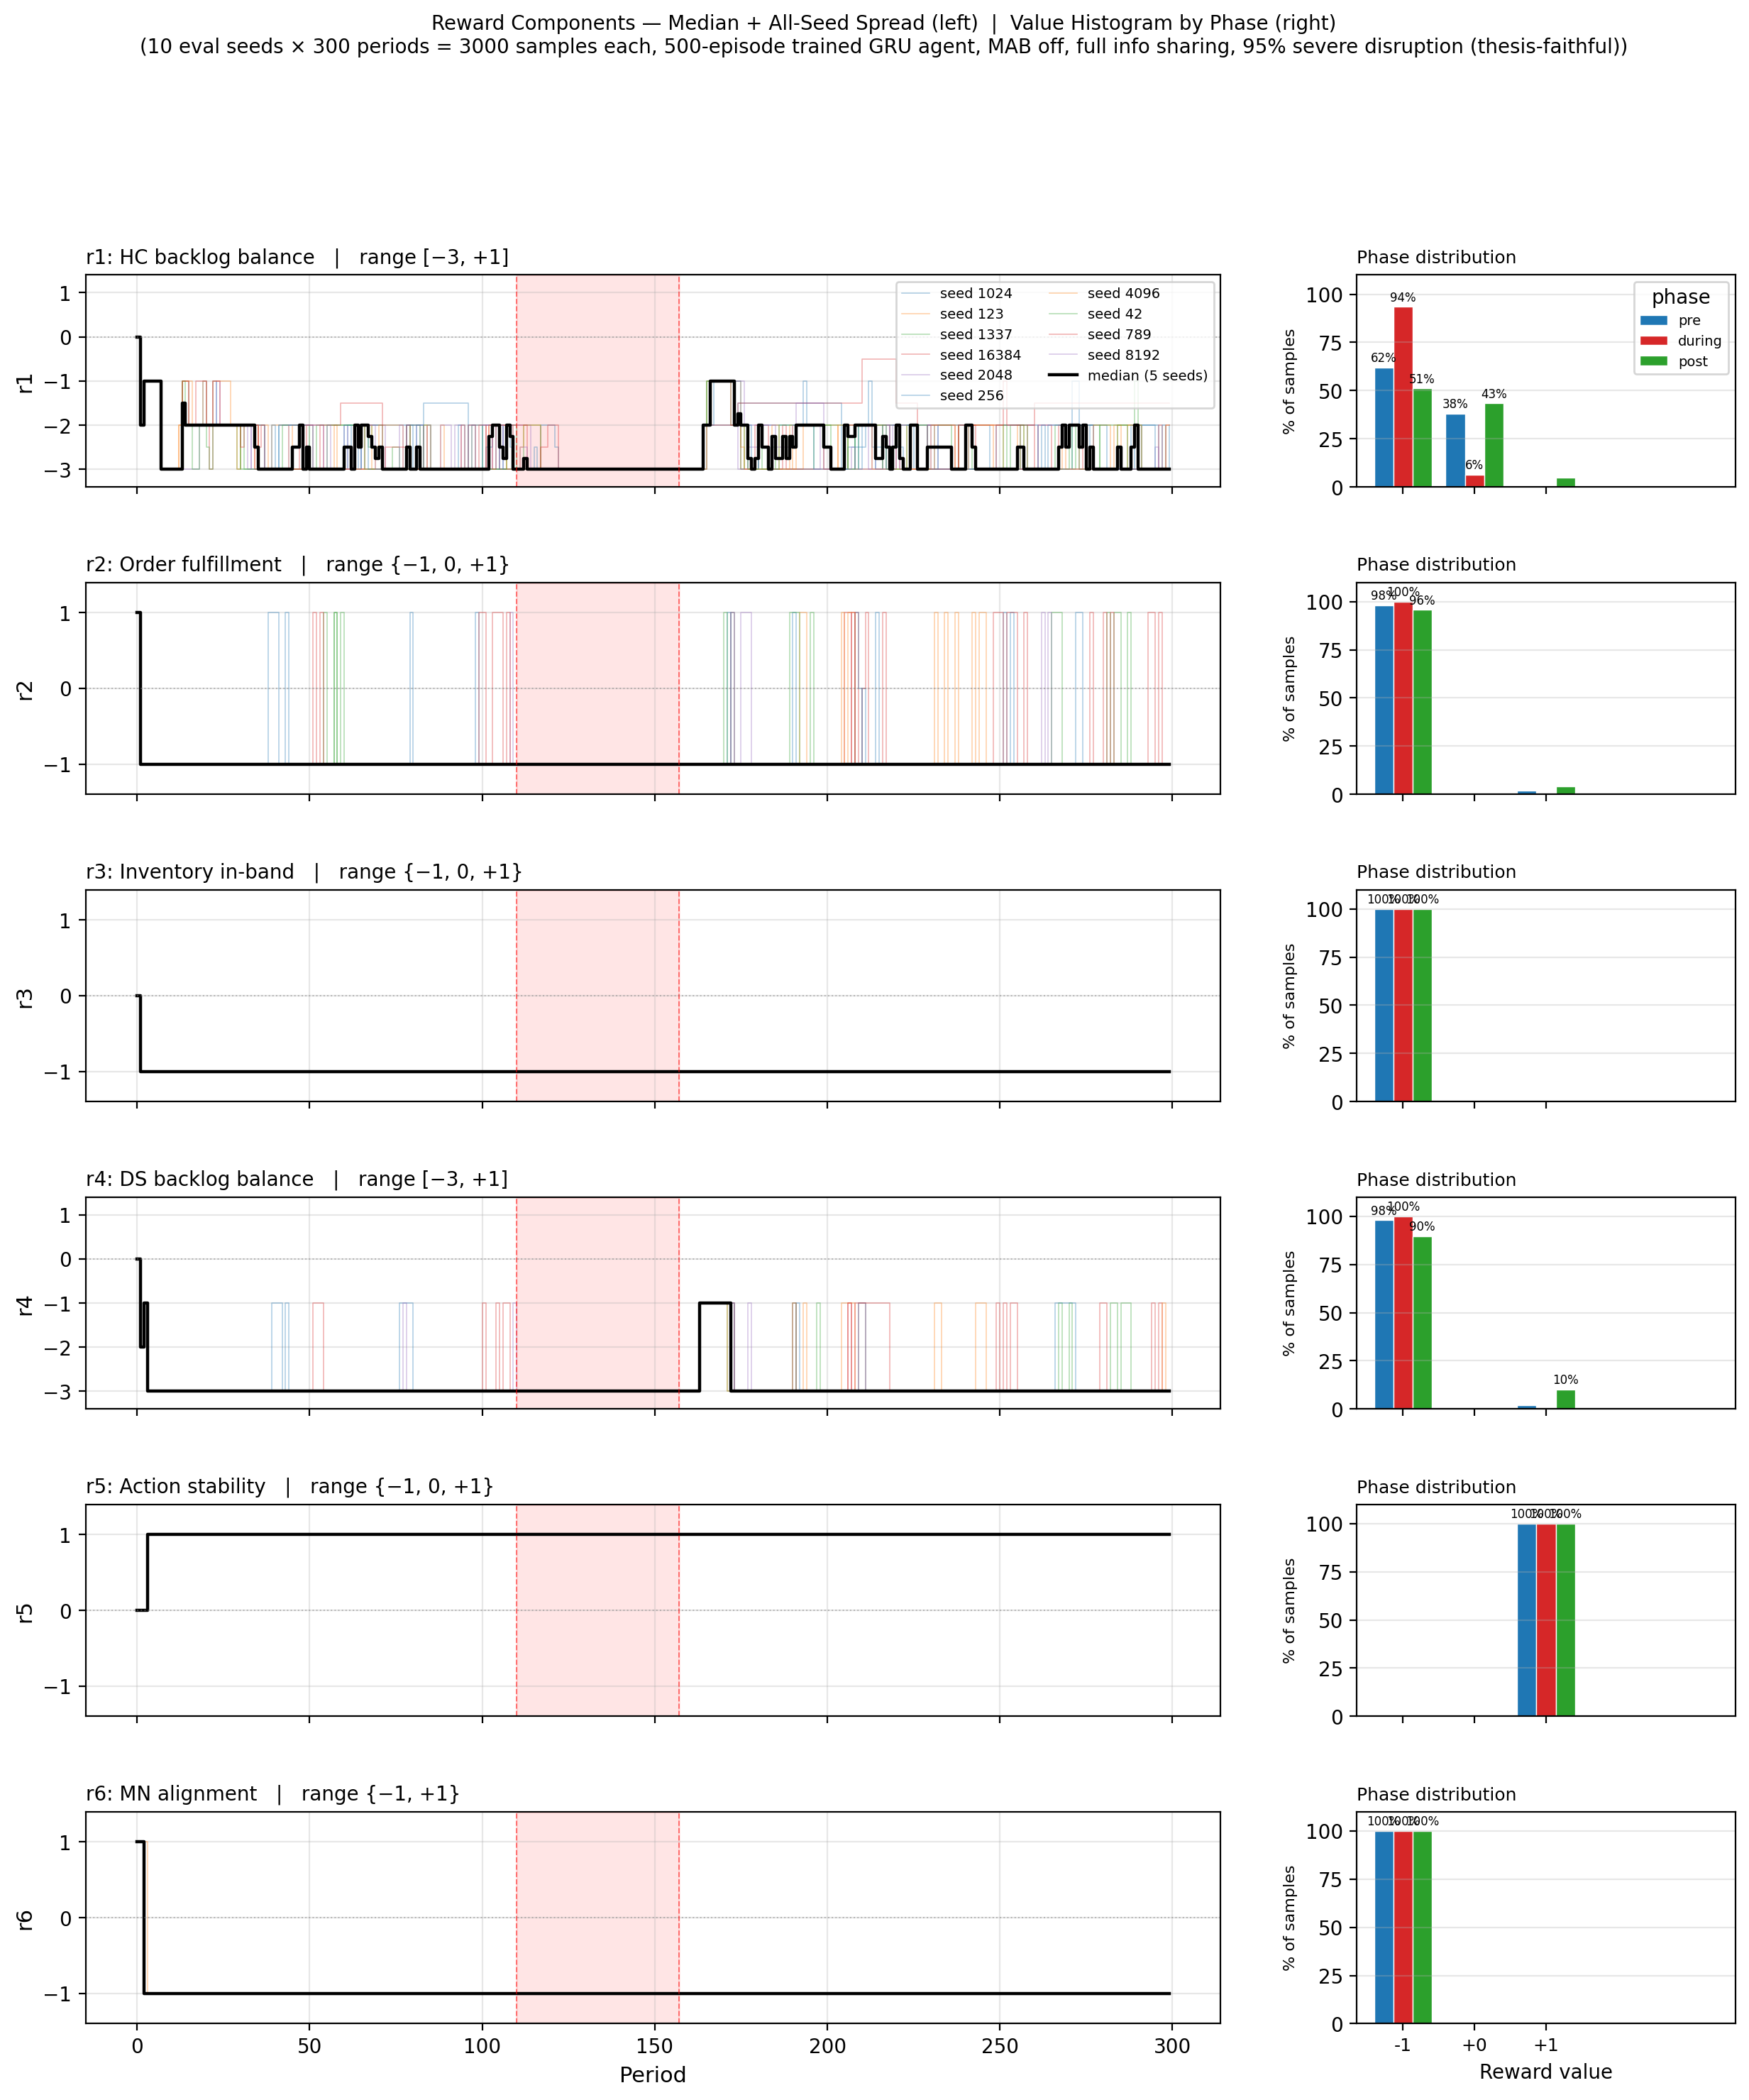
\includegraphics[width=\textwidth]{r5_test_results/reward_components_v2.png}
\caption{Reward components $r_1$--$r_6$: median time-series across 5 seeds with all-seed spread (left) and phase-conditional value distributions (right).  Disruption window 110--157 shaded red.  For $r_3$, $r_5$, $r_6$ the three phase bars are visually identical: the reward distribution is unchanged when the disruption fires.}
\label{fig:reward-components-v2}
\end{figure}

\section{Summary table of findings}

\begin{longtable}{p{0.06\linewidth} p{0.36\linewidth} p{0.40\linewidth} p{0.12\linewidth}}
\toprule
\textbf{$r_i$} & \textbf{Finding} & \textbf{Fix / Status} & \textbf{Effort} \\
\midrule
$r_1$ & Pinned in $\{-3,-2,-1\}$ by the Eq.~3.13 oscillation term --- a \textbf{thesis-level} algebraic flaw, faithfully implemented. & Count true reversals of $\Delta b$: change \code{abs(sign(diff){-}sign(-diff))} to \code{abs(sign(delta\_b[j+1]){-}sign(delta\_b[j]))}. & 1 line \\
\addlinespace
$r_4$ & Same inheritance from \code{\_compute\_backlog\_balance}. & Fixed by the $r_1$ change (shared helper). & 0 lines \\
\addlinespace
$r_5$ & Pinned at $+1$ because the slope is computed on the normalised order ratio $[0,1]$ instead of raw order quantity. & Author-confirmed \textbf{code fix}: store the raw order quantity at \code{last\_actions[i][0]} in \code{take\_actions()}. & 1 line \\
\addlinespace
$r_6$ & Constant $-1$.  Two issues: \textbf{(a)} all-or-nothing window pins $-1$ on first violation; \textbf{(b)} \textbf{structural} --- agent does not control \code{MN\_prod}, so the only available DS action that fixes $r_6$ during disruption is under-ordering --- a perverse incentive. & (a) Graded $\mathrm{sign}(n_{\text{in}}{-}n_{\text{out}})$. (b) Requires re-formulating the metric around something the DS actually controls. & 4 lines $+$ redesign \\
\addlinespace
$r_2$ & Saturated in this run, but plausibly driven by \emph{constant} patient demand $+$ the trained agent's under-ordering rather than by the reward formula. & \textbf{Defer.}  Re-evaluate with stochastic demand and a properly-trained agent. & --- \\
\addlinespace
$r_3$ & Saturated because constant demand collapses $\sigma_{S^*}$ to its code floor of $1.0$, giving a 2-unit band; not necessarily a design flaw in a stochastic-demand regime. & \textbf{Defer.}  Re-evaluate with stochastic demand. & --- \\
\bottomrule
\end{longtable}

\section{Open questions for the next meeting with Zoreh}

\begin{enumerate}
  \item Is there a corrected version of \code{\_compute\_backlog\_balance} (the Eq.~3.13 term2 issue) in your working copy that did not make it into the shared repo?  We did not find any reference to it in your reply about $r_5$.
  \item The thesis text does not describe the \code{DRL\_EQ1\_PROXY\_WEIGHT} term (default $0.15$ in code, applied as an additive penalty after the Eq.~3.9 sum).  Confirm: was it off during the thesis experiments, or was it on but undocumented?
  \item For $r_3$: was the up-to-level band ($\pm 2\sigma_{S^*}$) intended only against \emph{stochastic} patient demand, where $\sigma_{S^*}$ provides a meaningful scale?  Was the \code{PATIENT\_MODEL\_TYPE = constant} setup ever used in the thesis runs, or were the thesis runs always under stochastic demand?
  \item For $r_6$: the DS does not control \code{MN\_prod}, so during a disruption the only DS action that returns $r_6$ to $+1$ is under-ordering.  Is this intended (rewarding the DS for throttling during shortages), or was the metric intended to measure something the DS actually controls (e.g.\ DS-to-HC alignment) that got conflated with manufacturer production?
  \item The MAB was disabled here for isolation.  In your runs with MAB on, did the bandit consistently down-weight $r_5$ during normal operation and/or up-weight \emph{anti}-correlated arms during disruption?  Chapter~4 figures show arm~8 (halved $r_5$) frequently selected, which is consistent with the bandit compensating for $r_5$'s saturation at $+1$.
\end{enumerate}

\section*{Reproducibility}

All code is in the \code{Inventory\_DRL\_MAB-main} repository.  The diagnostic script is \code{run\_r5\_diagnostic.py} (entry point) which calls \code{gen\_reward\_components\_v2.py} for the figure above.  Eval data is in \code{r5\_test\_results/episode\_*\_DS1\_r5log.csv}.  The trained checkpoint (500 episodes, seed 42, MAB off, proxy off) is in \code{r5\_test\_results/checkpoint/}.  Re-running the eval-only path:
\begin{lstlisting}[language=bash]
python3 run_r5_diagnostic.py --skip-train
\end{lstlisting}

\end{document}
